\section{Optimisation}\label{sec:optimisation}
In this section, we study optimisation with fixed NPFs, i.e., a setting in which $\ip{\partial \phi,v}=0$. Here, we are interested in learning: $\hat{y}_t(x)=\ip{\phi_{x,0}, v_t}$, which boils down to learning the NPVs $v_t$. To this end, we use the DGN framework, wherein, the gating network provides the fixed NPFs and training the value network will learn the NPVs.
\begin{assumption}\label{assmp:main}
(i) $\Theta_0\inrdnet$ is statistically independent of NPFs, (ii) $\Theta_0$ are sampled i.i.d from a distribution such that for any $\theta_0\in\Theta_0$,  we have $\E{\theta_0}=0$, and  $\E{\theta^2_0}=\sigma^2$, and $\E{\theta^4_0}={\sigma'}^2$.
\end{assumption}
\begin{theorem}[\textbf{Main Result}]\label{th:main} Under \Cref{assmp:main}, we have:\\
(i) $\E{K_0}=d\sigma^{2(d-1)} H_0=d\sigma^{2(d-1)} (x^\top x)\odot \lambda_0$.\\
(ii) In addition, if ${4d}/{w^2}<1$, then $Var\left[K_0\right]\leq O\left(d^2_{in}\sigma^{4(d-1)}\max\{d^2w^{2(d-2)+1}, d^3w^{2(d-2)}\}\right)$.
\end{theorem}
\begin{comment}
\begin{lemma}\label{lm:disentangle}[Disentanglement] Let $\nabla_{\Theta} v_t\in \R^{P\times d_{net}}$ be matrix whose entries are given by $\nabla_{\Theta} v_t (p,\theta)=\partial_{\theta}v_t(p),\forall p\in [P], \theta\in\Theta$, and let $I_P$ be the $P\times P$ identity matrix. Then, 
under \Cref{assmp:main}-(ii), it follows that $\E{\nabla_{\Theta}v_{\Theta_t})(\nabla_{\Theta}v_{\Theta_t})^\top }= d\sigma^{2(d-1)}I_{P}$.
\end{lemma}
\begin{comment}
\textbf{Proof of \Cref{th:main}-(i):} Let $\varphi_t=(\varphi_{p,t},p\in[P])\in \R^{d_{net}\times P}$ matrix, then since $K_t=\Psi^\top_t\Psi$, where $\Psi_t=\varphi_t \Phi_t$, we have $\E{K_t}=\E{\Phi^\top_t \varphi^\top_t \varphi_t \Phi_t}$. At initialisation, using the \Cref{assmp:main}-(i), we can pull out $\Phi^\top_t$ and $\Phi_t$ outside of the expectation to have \begin{align}\label{eq:pullout}\E{K_0}=\Phi^\top_0\E{ \varphi^\top_t \varphi_t }\Phi_0,\end{align} and from \Cref{lm:disentangle}, it follows that $\E{ \varphi^\top_t \varphi_t }=d\sigma^{2(d-1)}I$, and hence $\E{K_0}=d\sigma^{2(d-1)}\Phi^\top_0\Phi_0=d\sigma^{2(d-1)}H_0$.\\
\end{comment}
%This overlap is captured by $\lambda_t(s,s')$ which is the measure of overlap of the sub-networks that are active for both the inputs $x,x'\in\R^{d_{in}}$. Under. \Cref{assmp:main}, the inter-path interaction $\varphi^\top_t\varphi_t$ gets disentangled, result in the claim \Cref{th:main}-(i).\\
%However, in the later part of this section, we consider a special case, wherein, we give an explicit characterisation of the spectrum of $\E{K_0}$. Characterising $\lambda_0$ for the general case is left as future work.\\
\textbf{Why increasing depth till a point helps in training? } Let us first look at the diagonal terms of $\lambda_0$. It is reasonable to assume that, owing to the symmetric nature of the weights, roughly $\mu=\frac{1}{2}$ fraction of the gates are \emph{on} every layer. Thus $\lambda_0(s,s)\approx (w/2)^{d-1}$. Now, due our choice of $\sigma=\sqrt{\frac{2}{w}}$, the diagonal entries will be close to $1$. We now turn our attention towards the non-diagonal entries of $\lambda_0$. Define $\tau(s,s',l)\stackrel{def}=\sum_{i=1}^w G_{x_s,t}(l,i)G_{x_{s'},t}(l,i)$ be the overlap of the active gates in layer $l$ for input examples $s,s'\in[n]$, and  let $\eta\stackrel{def}=\max_s\left(\max_{s',l} \frac{\tau(s,s',l)}{\tau(s,s,l)}\right)$ be the maximum overlap between gates of a layer (maximum taken over over input pairs $s,s'\in[n]$ and layers $l\in [d]$).  Then it follows that $\max_{s,s'\in [n]} \frac{\bar{\lambda}_{cross}(s,s')}{\bar{\lambda}_{self}(s)}\leq \eta^{d-1}$. Thus, the non-diagonal entries decay an exponential rate in comparison to the diagonal entries.\hfill\\
\textbf{Why increasing the depth beyond hurts training?} The variance expression in \Cref{th:main}-$(ii)$ involves $d^2$ and $d^3$ terms, and hence for a fixed width as depth increases, the entries of $K_0$ deviates from $\E{K_0}$, and as a result the spectrum of $K_0$ degrades, thereby hurting training performance.\\
\textbf{Characterising $\lambda_0$:} Note that $\lambda_0$ is the matrix of correlation of the active sub-network for each input, and thus $\lambda_0$ depends on the inputs. However, what we have argued is that this input dependence of $\lambda_0$ \emph{fades} away as the depth increases. However, for a general dataset, it is not possible to further comment on the spectral properties of $\lambda_0$. In what follows, we look an experiment, wherein, we completely control $\lambda_0$ so as to gain further insights.
\begin{comment}$5.$ \Cref{assmp:main} is not satisfied by ReLU activations, i.e., conditioned on the fact that a ReLU is \emph{on}, the incoming weights cannot all be simultaneously negative. This implies that the $\Phi^\top_t$ and $\Phi_t$ terms cannot be pulled out of the expectation as in \eqref{eq:pullout}.
\end{comment}
\begin{comment}
\begin{wrapfigure}{h}{0.27\textwidth}
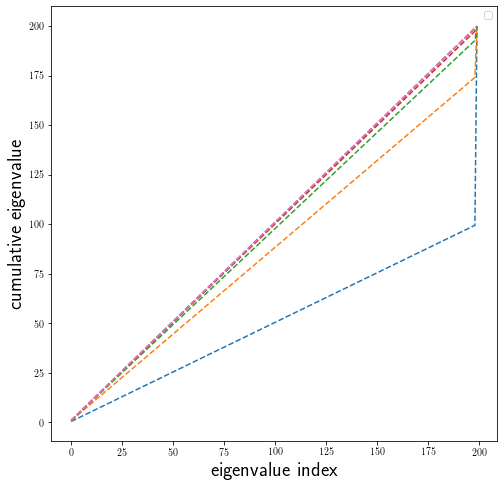
\includegraphics[scale=0.22]{figs/dgn-fra-ecdf-ideal.png}
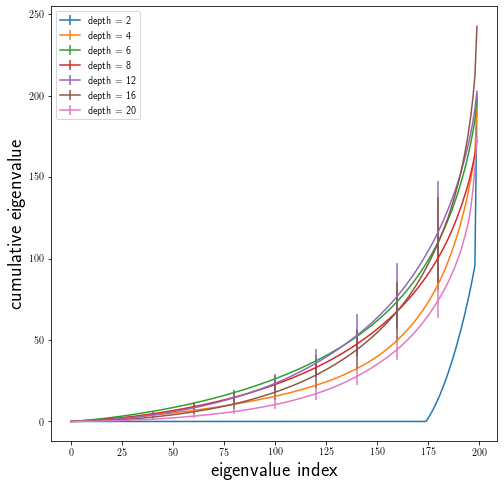
\includegraphics[scale=0.22]{figs/dgn-fra-ecdfbyd-w25.png}
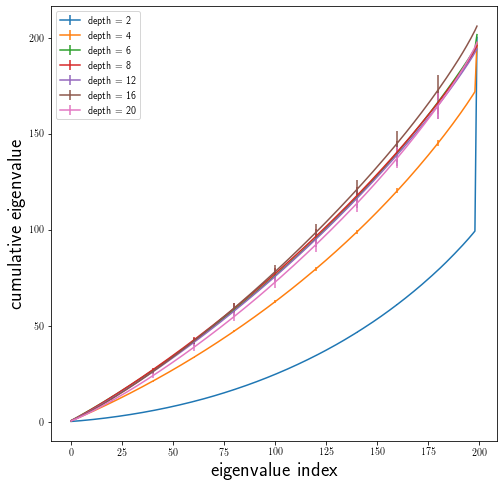
\includegraphics[scale=0.22]{figs/dgn-fra-ecdfbyd-w500.png}
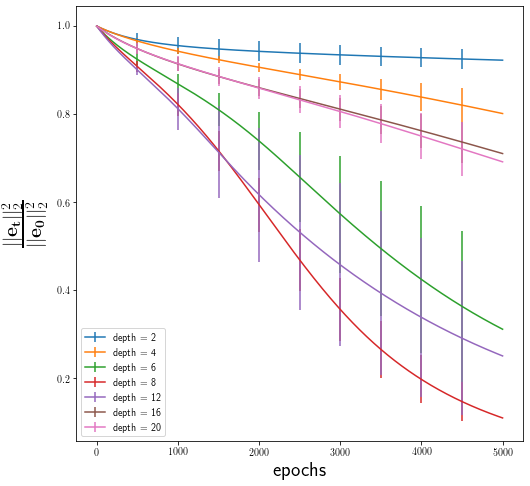
\includegraphics[scale=0.21]{figs/dgn-fra-conv-w25.png}
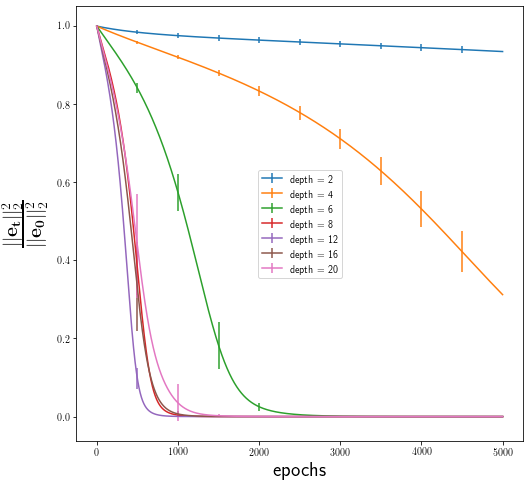
\includegraphics[scale=0.21]{figs/dgn-fra-conv-w500.png}
\caption{Ideal spectrum}
\label{fig:dgn-frg-gram-ecdf}
\end{wrapfigure}
\end{comment}
\begin{comment}
\textbf{A:} In our experiment, we consider DGNs with the following three different gating schemes namely, i) fixed random (FR): for each input example in the dataset, we sample gating values from $Ber(\mu)$ taking values in $\{0,1\}$, and collect it in $\G_0$. DGN with FR gating is useful only for pure memorisation, ii) fixed explicit (FE): gating parameter $\Tg_t=\Tg_0,\forall\, t\geq 0, \Tg_0\neq \Theta_0$, iii) fixed implicit (FI): gating parameter $\Tg_t=\Tg_0,\forall\, t\geq 0, \Tg_0= \Theta_0$. The FI case does not satisfy \Cref{assmp:main}-(i).
\end{comment}
\begin{wrapfigure}{h}{0.20\textwidth}
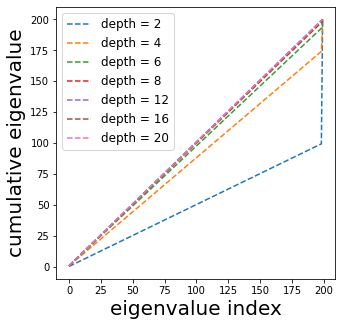
\includegraphics[scale=0.2]{figs/dgn-fra-ecdf-ideal-small.png}
\caption{Ideal spectrum.}
\label{fig:ideal-spectrum}
\end{wrapfigure}
\textbf{Experiment with fixed random gates:} We consider the dataset given by $(x_s,y_s)_{s=1}^n\in \R\times \R$, where $x_s=1,\forall s\in [n]$, and $y_s\sim unif([-1,1])$, $n=200$. For each input example in the dataset, we sample gating values from $Ber(\mu)$ taking values in $\{0,1\}$, and collect it in $\G_0$, which we keep fixed throughout training of the DGN (i.e., $\G_t=\G_0,\,\forall\,t\geq 0$).  Even though the input is the same for all the $n$ examples, via the fixed random gating strategy, we ensure that there is a separate random sub-network for each input example.  In this case, it is easy to check that $\mathbb{E}_{\mu}\left[\lambda_0(s,s)\right]=(\mu w)^{(d-1)},\forall s\in[n]$ and $\mathbb{E}_{\mu}\left[\lambda_0(s,s')\right]=(\mu^2 w)^{(d-1)},\forall s,s'\in[n]$.\WFclear
$\bullet$ \textbf{Spectrum (Ideal):} The input Gram matrix $x^\top x$ is a $n\times n$ matrix with all entries equal to $1$ and its rank is equal to 1, and hence $H_0=\lambda_0$.  For $\sigma=\sqrt{\frac{1}{\mu w}}$, and by further averaging $\mathbb{E}_{\mu}\left[K_0(s,s)/d\right]=1$, and $\mathbb{E}_{\mu}\left[K_0(s,s')/d\right]=\mu^{(d-1)}$. Now, let $\rho_i\geq 0,i \in [n]$ be the eigenvalues of $\frac{\E{K_0}}{d}$, and let $\rho_{\max}$ and $\rho_{\min}$ be the largest and smallest eigenvalues.  One can easily show that $\rho_{\max}=1+(n-1)\mu^{d-1}$ and corresponds to the eigenvector with all entries as $1$, and $\rho_{\min}=(1-\mu^{d-1})$ repeats $(n-1)$ times,  which corresponds to eigenvectors given by $[0, 0, \ldots, \underbrace{1, -1}_{\text{$i$ and $i+1$}}, 0,0,\ldots, 0]^\top \in \R^n$ for $i=1,\ldots,n-1$. Note that as $d\ra\infty$, $\rho_{\max},\rho_{\min}\ra 1$.\\
$\bullet$ \textbf{Spectrum (numerical):} We look at the cumulative eigenvalue (e.c.d.f) obtained by first sorting the eigenvalues in ascending order then looking at their cumulative sum. The ideal behaviour (top plot of \Cref{fig:dgn-frg-gram-ecdf}) as predicted from theory is that for indices $k\in[n-1]$, the e.c.d.f should increase at a linear rate, i.e., the cumulative sum of the first $k$ indices is equal to $k(1-\mu^{d-1})$, and the difference between the last two indices is $1+(n-1)\mu^{d-1}$. In \Cref{fig:dgn-frg-gram-ecdf}, we plot the actual e.c.d.f for various depths $d=2,4,6,8,12,16,20$ and $w=25,500$ a (second and third from top in \Cref{fig:dgn-frg-gram-ecdf}). \hfill\\
$\bullet$ \textbf{Convergence (numerical):} In order to compare how the rate of convergence varies with the depth, we set the step-size $\alpha=\frac{0.1}{\rho_{\max}}$, $w=100$. We use the vanilla SGD-optimiser. Note the$ \frac{1}{\rho_{\max}}$ in the stepsize, ensures that the uniformity of maximum eigenvalue across all the instances, and the convergence should be limited by the smaller eigenvalues. We also look at the convergence rate of the ratio $\frac{\norm{e_t}^2_2}{\norm{e_0}^2_2}$. We notice that for $w=25$, increasing depth till $d=8$ improves the convergence, however increasing beyond $d=8$ worsens the convergence rate. For $w=500$, increasing the depth till $d=12$ improves convergence, and $d=16,20$ are worse than $d=12$.  This matches with the depth phenomena observed in practical DNNs and also matches our theory.
\begin{figure*}[!b]
\resizebox{\textwidth}{!}{
\begin{tabular}{cccc}
%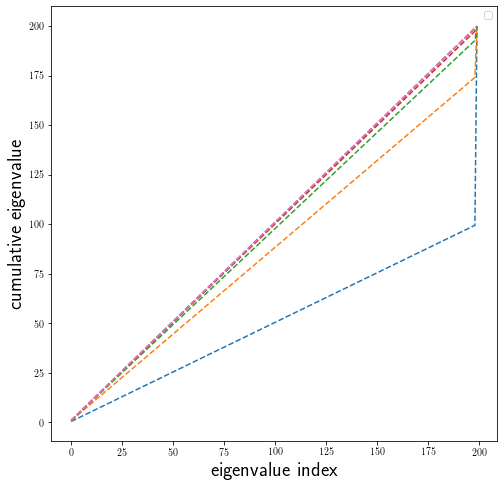
\includegraphics[scale=0.4]{figs/dgn-fra-ecdf-ideal.png}
%&
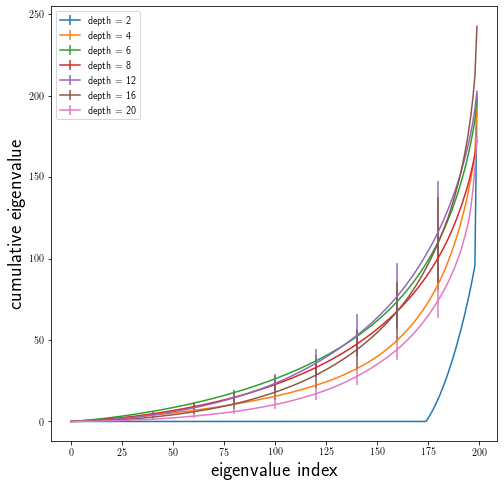
\includegraphics[scale=0.5]{figs/dgn-fra-ecdfbyd-w25.png}
&
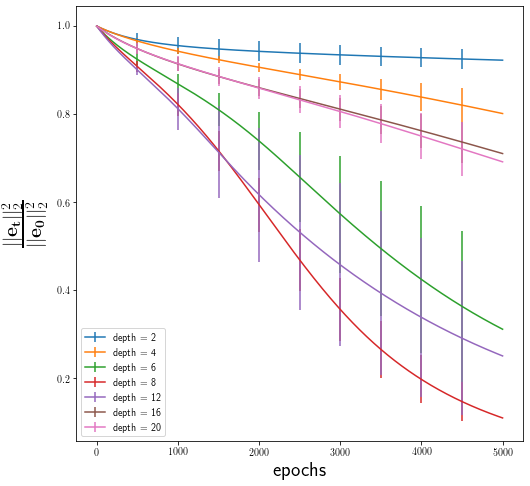
\includegraphics[scale=0.5]{figs/dgn-fra-conv-w25.png}
&
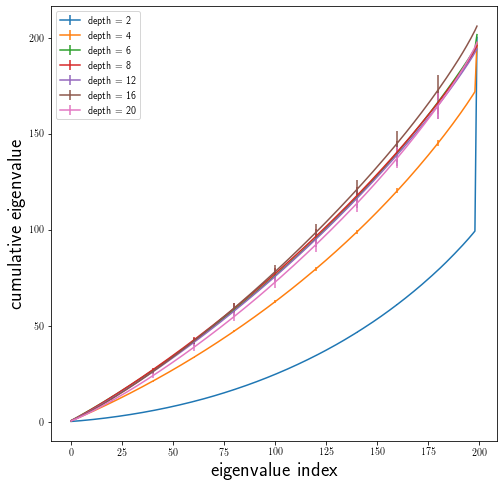
\includegraphics[scale=0.5]{figs/dgn-fra-ecdfbyd-w500.png}
&
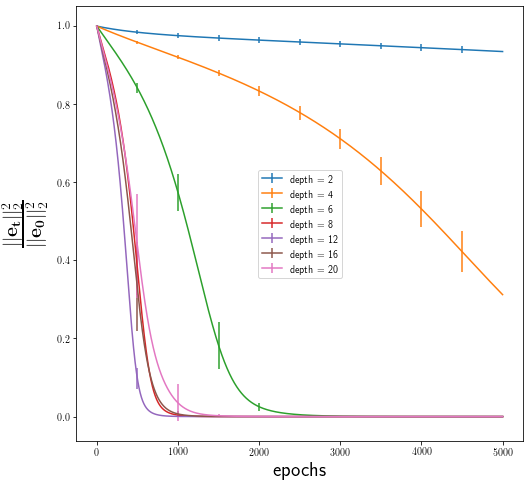
\includegraphics[scale=0.5]{figs/dgn-fra-conv-w500.png}
\end{tabular}
}
\caption{Shows the plots for fixed random gating with $\mu=\frac{1}{2}$ and $\sigma=\sqrt{\frac{2}{w}}$. }
\label{fig:dgn-frg-gram-ecdf}
\end{figure*}

\begin{comment}
\begin{figure}
\resizebox{\textwidth}{!}{
\begin{tabular}{cccc}
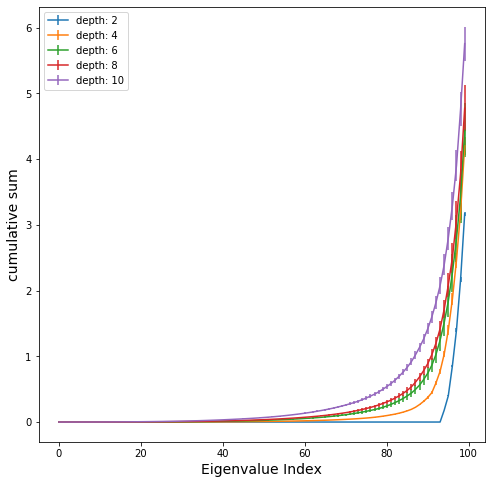
\includegraphics[scale=0.4]{figs/galu-ecdf-d.png}
&
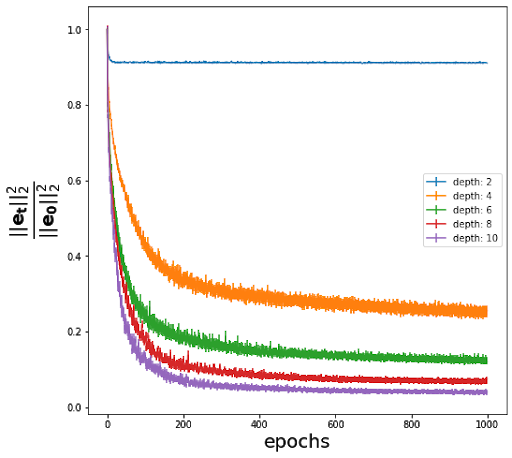
\includegraphics[scale=0.4]{figs/galu-conv-d.png}
&
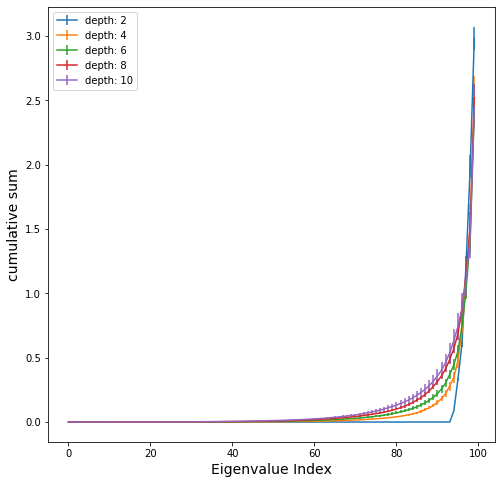
\includegraphics[scale=0.4]{figs/relu-ecdf.png}
&
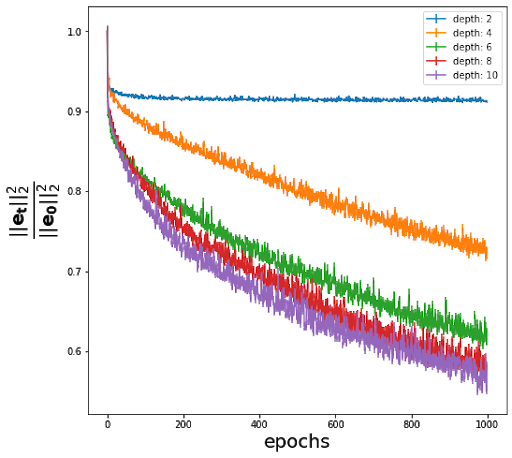
\includegraphics[scale=0.4]{figs/relu-conv.png}
\end{tabular}
}
\caption{The left two plots shows the e.c.d.f and convergence rates for various depth in GaLU networks $w=100$. The third and fourth plot from the left show the e.c.d.f and convergence rates for various depth in ReLU networks $w=100$. The plots are averaged over $5$ runs. }
\label{fig:galu-d}
\end{figure}
\end{comment}